\documentclass{article}
\usepackage[landscape]{geometry}
\usepackage{url}
\usepackage{multicol}
\usepackage{amsmath}
\usepackage{esint}
\usepackage{amsfonts}
\usepackage{tikz}
\usetikzlibrary{decorations.pathmorphing}
\usepackage{amsmath,amssymb}

\usepackage{colortbl}
\usepackage{xcolor}
\usepackage{mathtools}
\usepackage{amsmath,amssymb}
\usepackage{enumitem}
\makeatletter

\newcommand*\bigcdot{\mathpalette\bigcdot@{.5}}
\newcommand*\bigcdot@[2]{\mathbin{\vcenter{\hbox{\scalebox{#2}{$\m@th#1\bullet$}}}}}
\makeatother

\title{Electromagnetism Cheat Sheet}
\usepackage[brazilian]{babel}
\usepackage[utf8]{inputenc}

\advance\topmargin-1in
\advance\textheight3in
\advance\textwidth3in
\advance\oddsidemargin-1.5in
\advance\evensidemargin-1.5in
\parindent0pt
\parskip2pt
\newcommand{\hr}{\centerline{\rule{3.5in}{1pt}}}
%\colorbox[HTML]{e4e4e4}{\makebox[\textwidth-2\fboxsep][l]{texto}
\begin{document}

\begin{center}{\huge{\textbf{Electromagnetism}}}\\
\end{center}
\begin{multicols*}{3}

\tikzstyle{mybox} = [draw=black, fill=white, very thick,
    rectangle, rounded corners, inner sep=10pt, inner ysep=10pt]
\tikzstyle{fancytitle} =[fill=white, text=black, font=\bfseries]

%------------ Ampere's law  ---------------
\begin{tikzpicture}
\node [mybox] (box){%
    \begin{minipage}{0.3\textwidth}
$$
\oint_C \mathbf{B} \cdot d \mathbf{l}=\mu_0 I_{\mathrm{enc}} \quad \text { (magnetostatics), }
$$
$$
\begin{aligned}
|\mathbf{B}| \oint_C d l & =\mu_0 I_{\mathrm{enc}}, \\
|\mathbf{B}| & =\frac{\mu_0 I_{\mathrm{enc}}}{L},
\end{aligned}
$$
where $L$ is the length of the curve $C$. The dircetion is determine by the right hand rule:
    \centering
    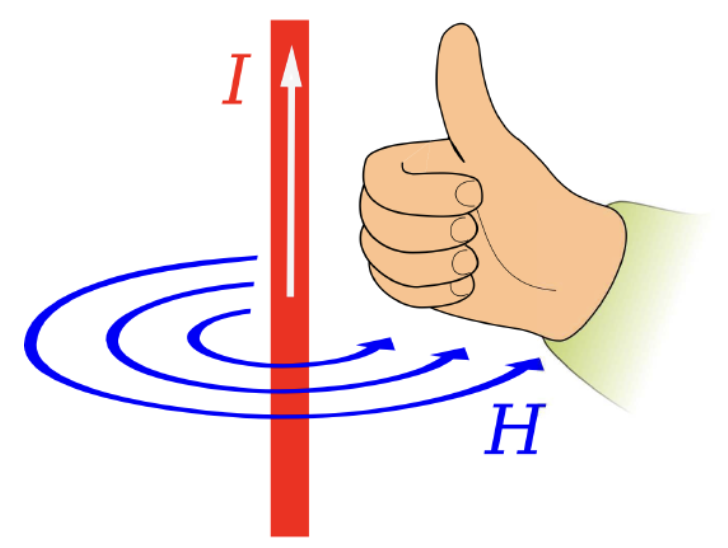
\includegraphics[width=0.6\linewidth]{right-hand-rule-mang.png}\\
    Put your thumb in the direction of the current, from the Biot-Savart law we know that the magnetic field is perpendicular to the current. the magnetic filed is the same direction of the curl of your fingers.
    
    \end{minipage}
};
%------------ Ampere's law Header ---------------------
\node[fancytitle, right=10pt] at (box.north west) {Ampere's law};
\end{tikzpicture}

%------------ Standard Magnetostatics Configurations Motion ---------------
\begin{tikzpicture}
\node [mybox] (box){%
    \begin{minipage}{0.3\textwidth}
    \begin{itemize}
        \item infinite wire
    \end{itemize}
    \centering
    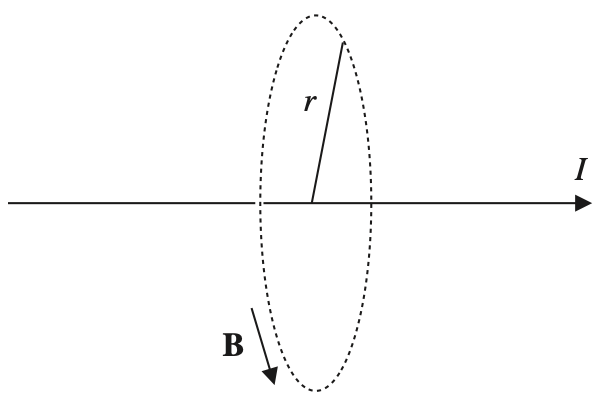
\includegraphics[width=0.6\linewidth]{infinite wire.png}
    \begin{itemize}
        \item Infinite sheet
    \end{itemize}
    \centering
    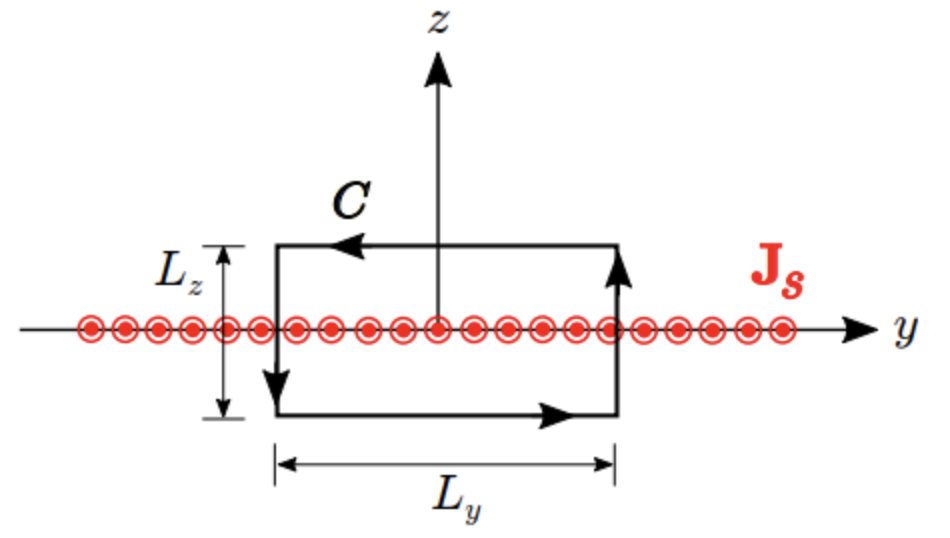
\includegraphics[width=0.8\linewidth]{infinite sheet.png}
    \begin{itemize}
        \item Toroidal coil
    \end{itemize}
    \centering
    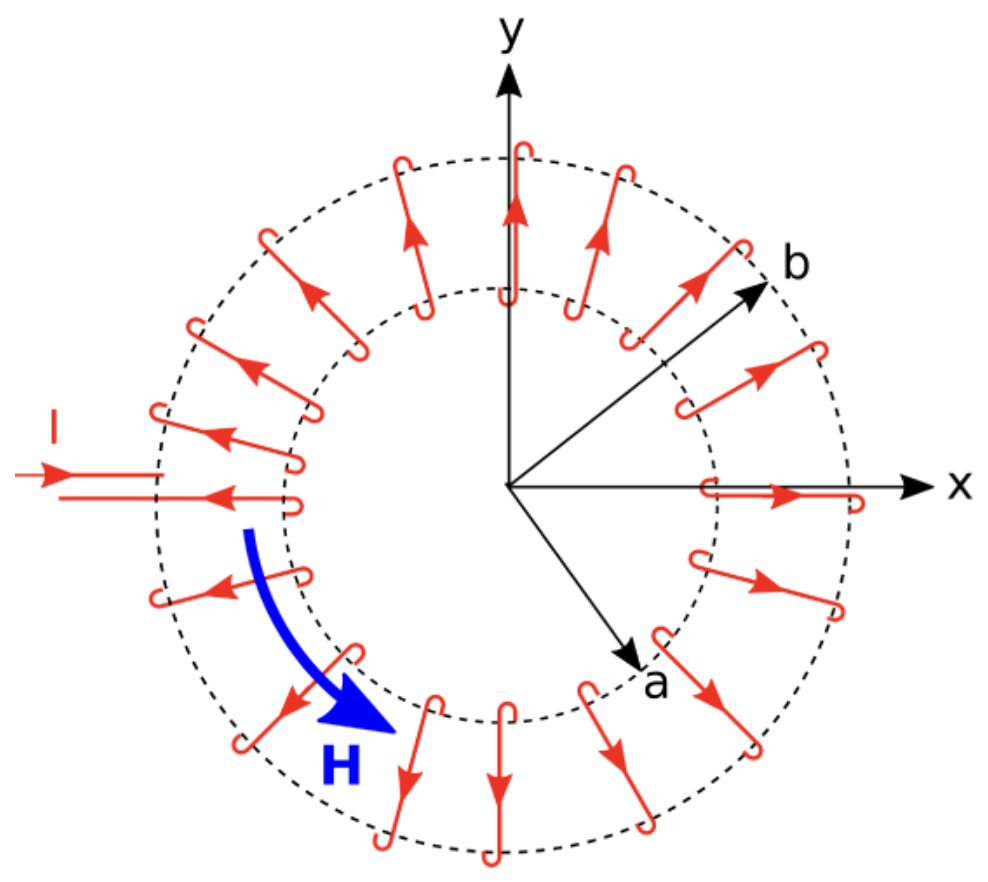
\includegraphics[width=0.7\linewidth]{toroidal coil.png}
    \end{minipage}
};
%------------ Standard Magnetostatics Configurations Header ---------------------
\node[fancytitle, right=10pt] at (box.north west) {Standard Magnetostatics Configurations};
\end{tikzpicture}

%------------  ---------------
\begin{tikzpicture}
\node [mybox] (box){%
    \begin{minipage}{0.3\textwidth}

    \end{minipage}
};
%------------  Header ---------------------
\node[fancytitle, right=10pt] at (box.north west) {TBK};
\end{tikzpicture}


\end{multicols*}
\end{document}


Contact GitHub API Training Shop Blog About
© 2016 GitHub, Inc. Terms Privacy Security Status Help